El desarrollo del proyecto se ha dividido en 7 fases discretas, descritas a continuación:
\begin{itemize}
    \item \textbf{Fase 0: Consolidación de la idea y estudio de mercado}. El primer paso ha sido identificar el problema a resolver con la aplicación, e investigar las soluciones que existen en el mercado, tanto para ver cómo afrontan el problema, como para identificar puntos fuertes y puntos de dolor.
    \item \textbf{Fase 1: Definición de funcionalidades y primeros diseños}. Se generó un listado de funcionalidades que debe tener la aplicación para ofrecer la experiencia deseada. Se clasifican las funcionalidades en básicas, avanzadas esenciales, y avanzadas opcionales. Adicionalmente, se dividen según la entidad principal con la que operan. Tras definir las funcionalidades, se dibujaron mockups definiendo las distintas pantallas y la distribución de elementos en las mismas. 
    \item \textbf{Fase 2: Implementación de funcionalidades por entidad}. Se desarrollaron las funcionalidades descritas, implementando todas las funcionalidades básicas de una entidad antes de empezar a implementar funcionalidades de otra entidad. Una vez todas las funcionalidades básicas fueron implementadas, se hizo una segunda pasada desarrollando las funcionalidades avanzadas esenciales y opcionales.
    \item \textbf{Fase 3: Control de calidad}. Se desarrollaron pruebas automáticas, y se realizaron análisis con SonarQube para identificar y subsanar vulnerabilidades y problemas de mantenibilidad o complejidad.
    \item \textbf{Fase 4: Dockerización, CI/CD, despliegue}. Se configuró el entorno de Azure para permitir el despliegue, junto con los workflows de CI/CD encargados de realizar el mismo, y las configuraciones de docker necesarias para el empaquetado de la aplicación.
    \item \textbf{Fase 5: Escritura de la memoria}. Se ha redactado el presente documento recogiendo todo el proceso de desarrollo del proyecto.
    \item \textbf{Fase 6: Preparación de la presentación}. Se ha redactado una presentación de PowerPoint y llevado a cabo otras preparaciones necesarias para la defensa del proyecto ante un tribunal.
\end{itemize}

Aunque las fases se describen como pasos discretos y unidireccionales, tales que cuando uno se completa se pasa al siguiente, la realidad no ha sido puramente así. Las fases y fechas planteadas indican los periodos dedicados principalmente a cada tarea, pero no descuentan que se pudieran llevar a cabo tareas puntuales o ajustes menores propios de otras fases. 

\begin{figure}[H]
    \centering
    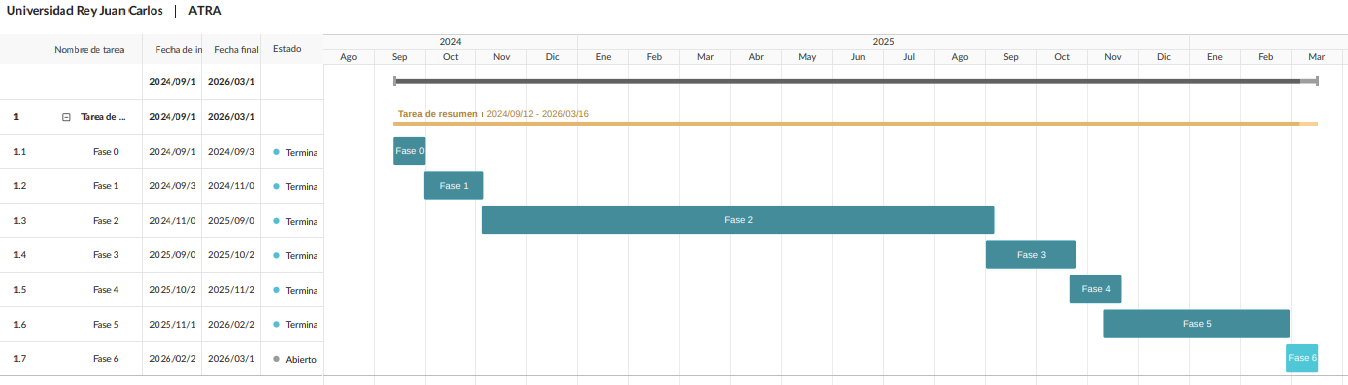
\includegraphics[width=1\linewidth]{img/gantt2.png}
    \caption{Diagrama de Gantt mostrando el flujo de trabajo}
    \label{fig:gantt}
\end{figure}

La figura \ref{fig:gantt} muestra la distribución del tiempo dedicado a cada fase del proyecto. Las fechas de la fase 6, así como la fecha final de la fase 5 son estimaciones, dado que estas fases no han terminado todavía.